%%%%%%%%%%%%%%%%%%%%%%%%%%%%%%%%%%%%%%%%%
% University/School Laboratory Report
% LaTeX Template
% Version 3.1 (25/3/14)
%
% This template has been downloaded from:
% http://www.LaTeXTemplates.com
%
% Original author:
% Linux and Unix Users Group at Virginia Tech Wiki 
% (https://vtluug.org/wiki/Example_LaTeX_chem_lab_report)
%
% License:
% CC BY-NC-SA 3.0 (http://creativecommons.org/licenses/by-nc-sa/3.0/)
%
%%%%%%%%%%%%%%%%%%%%%%%%%%%%%%%%%%%%%%%%%

%----------------------------------------------------------------------------------------
%	PACKAGES AND DOCUMENT CONFIGURATIONS
%----------------------------------------------------------------------------------------

\documentclass{article}

\usepackage[version=3]{mhchem} % Package for chemical equation typesetting
\usepackage{siunitx} % Provides the \SI{}{} and \si{} command for typesetting SI units
\usepackage{graphicx} % Required for the inclusion of images
\usepackage{natbib} % Required to change bibliography style to APA
\usepackage{amsmath} % Required for some math elements 

\setlength\parindent{0pt} % Removes all indentation from paragraphs

\renewcommand{\labelenumi}{\alph{enumi}.} % Make numbering in the enumerate environment by letter rather than number (e.g. section 6)

%\usepackage{times} % Uncomment to use the Times New Roman font

%----------------------------------------------------------------------------------------
%	DOCUMENT INFORMATION
%----------------------------------------------------------------------------------------

\title{Titanic: Machine Learning from Disaster \\ EECS 510} % Title

\author{Xiaoyang \textsc{Tan} \\ Zhaoyang \textsc{Liu} } % Author name


\date{\today} % Date for the report

\begin{document}
\maketitle
% If you wish to include an abstract, uncomment the lines below
% \begin{abstract}
% Abstract text
% \end{abstract}

%----------------------------------------------------------------------------------------
%	SECTION 1
%----------------------------------------------------------------------------------------

\section{Current work}

\subsection{Defining the problem}

\label{definitions}
	Information is given on a training set of passengers of the Titanic, for which the survival outcome is known. Given the training set information, the challenge is to predict each passenger?s survival outcome from a test set of passengers. The details of the challenge are given on the Kaggle site.
\newline
\newline
We will apply machine learning tools to solve the problem. In this case, we may consider approaches based on random forests. And will use Python package to plot the result. The python package used includes:
\begin{itemize}
	\item NumPy
	\item Pandas
	\item SciKit-Learn
	\item SciPy
	\item StatsModels
	\item Patsy
	\item Matplotlib
\end{itemize}
 


\subsection{Analyze the data}
In the training dataset, there are 891 passengers. Each passenger has 12 attributes. Except the "passangerId" and "Survived" attribute, we need to consider 10 other attributes 
and predict the survival possibility.

\subsubsection{Take care of missing values}
The features \textit{Ticket} and \textit{Cabin} have many missing values and so can?t add much value to our analysis. To handle this we will drop them from the data frame to preserve the integrity of our dataset. What's more, we will remove NaN values from every remaining column. Using \textbf{drop()} and \textbf{dropna()} function in could easily achieve goal. Now we have a clean and tidy dataset that is ready for analysis, we cut the dataset from 891 to 712, and get 8 effective attributes to do prediction.

\subsubsection{Graphical view of data}
The point of this competition is to predict if an individual will survive based on the features in the data like:
\begin{itemize}
	\item Traveling Class (called pclass in the data)
	\item Sex
	\item Age
\end{itemize}




\begin{figure}[h]
\begin{flushleft}
\hspace*{-1.2in}
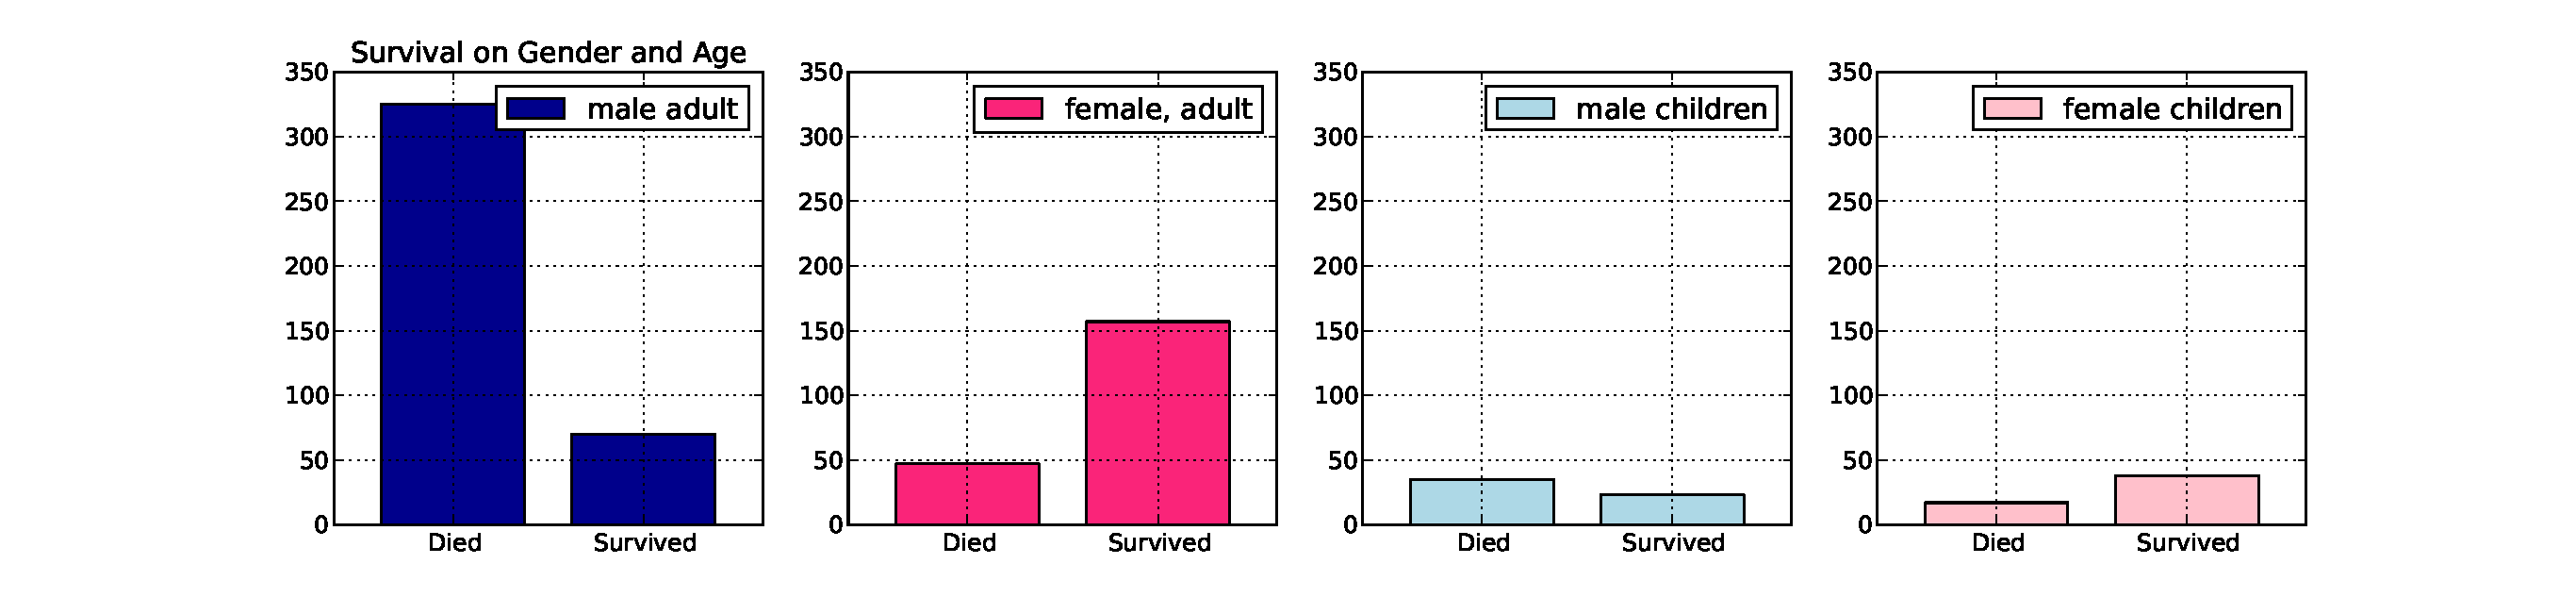
\includegraphics[scale=0.4]{eps/survival_gender_age.eps} % Include the image placeholder.png
\hspace*{-1.2in}
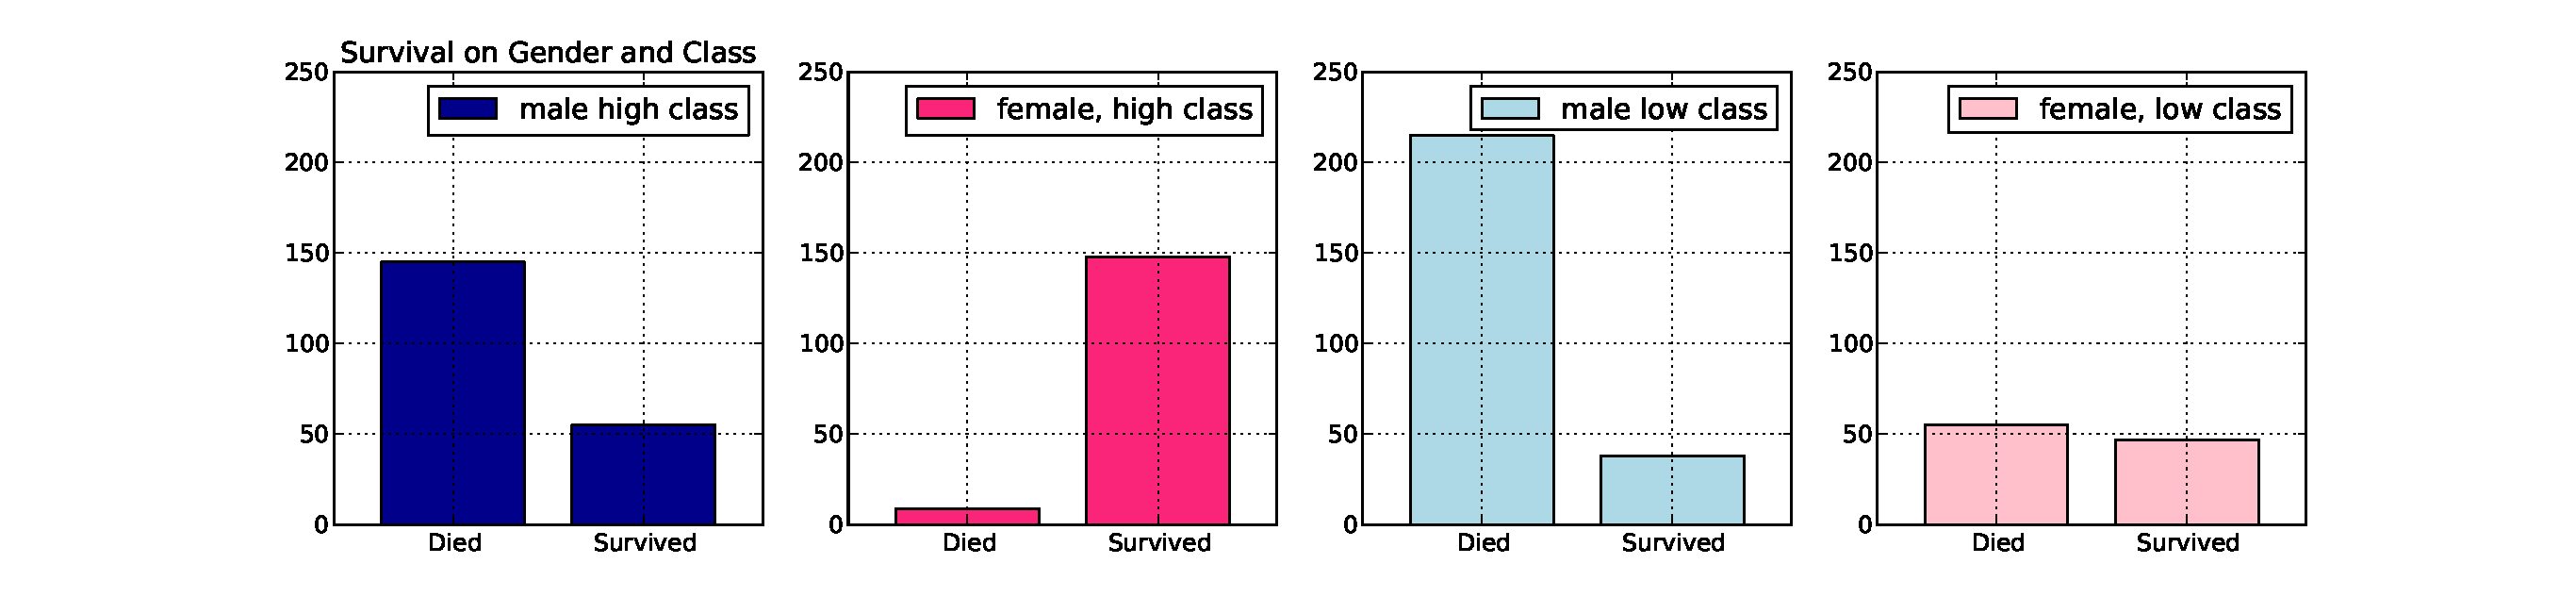
\includegraphics[scale=0.4]{eps/survival_gender_class.eps} 
\caption{Survival on gender, age and class}
\label {fig:test}
\end{flushleft}
\end{figure}

Figure~\ref{fig:test} shows the distribution of survival on gender age and class. ******


\subsection{Simple trying}
Simply pick gender as classfier and get the result.

\subsection{Supervised machine learning}


%----------------------------------------------------------------------------------------
%	SECTION 2
%----------------------------------------------------------------------------------------

\section{Next step}

\subsection{SVM}

\subsection{Random Forest}


%----------------------------------------------------------------------------------------
%	SECTION 3
%----------------------------------------------------------------------------------------


\section{Possible results}





\end{document}